\label{5_resultados}

\section{Parâmetros analisados}

Foram escolhidos parâmetros simples para analisar a evolução feita ao longo das gerações:

\begin{itemize}
	\item Valor mínimo de fitness em um indivíduo;
	\item Valor máximo de fitness em um indivíduo;
	\item Valor médio de fitness entre todos os indivíduos;
	\item Desvio padrão dos valores de fitness.
\end{itemize}

O desvio padrão aqui foi calculado por:

\begin{equation}
	\sigma = \sqrt{\frac{1}{N-1} \sum_{i=1}^N (x_i - \overline{x})^2}
\end{equation}

\section{OneMax Booleano}

Texto.

\begin{figure}[ht!]
    \centering 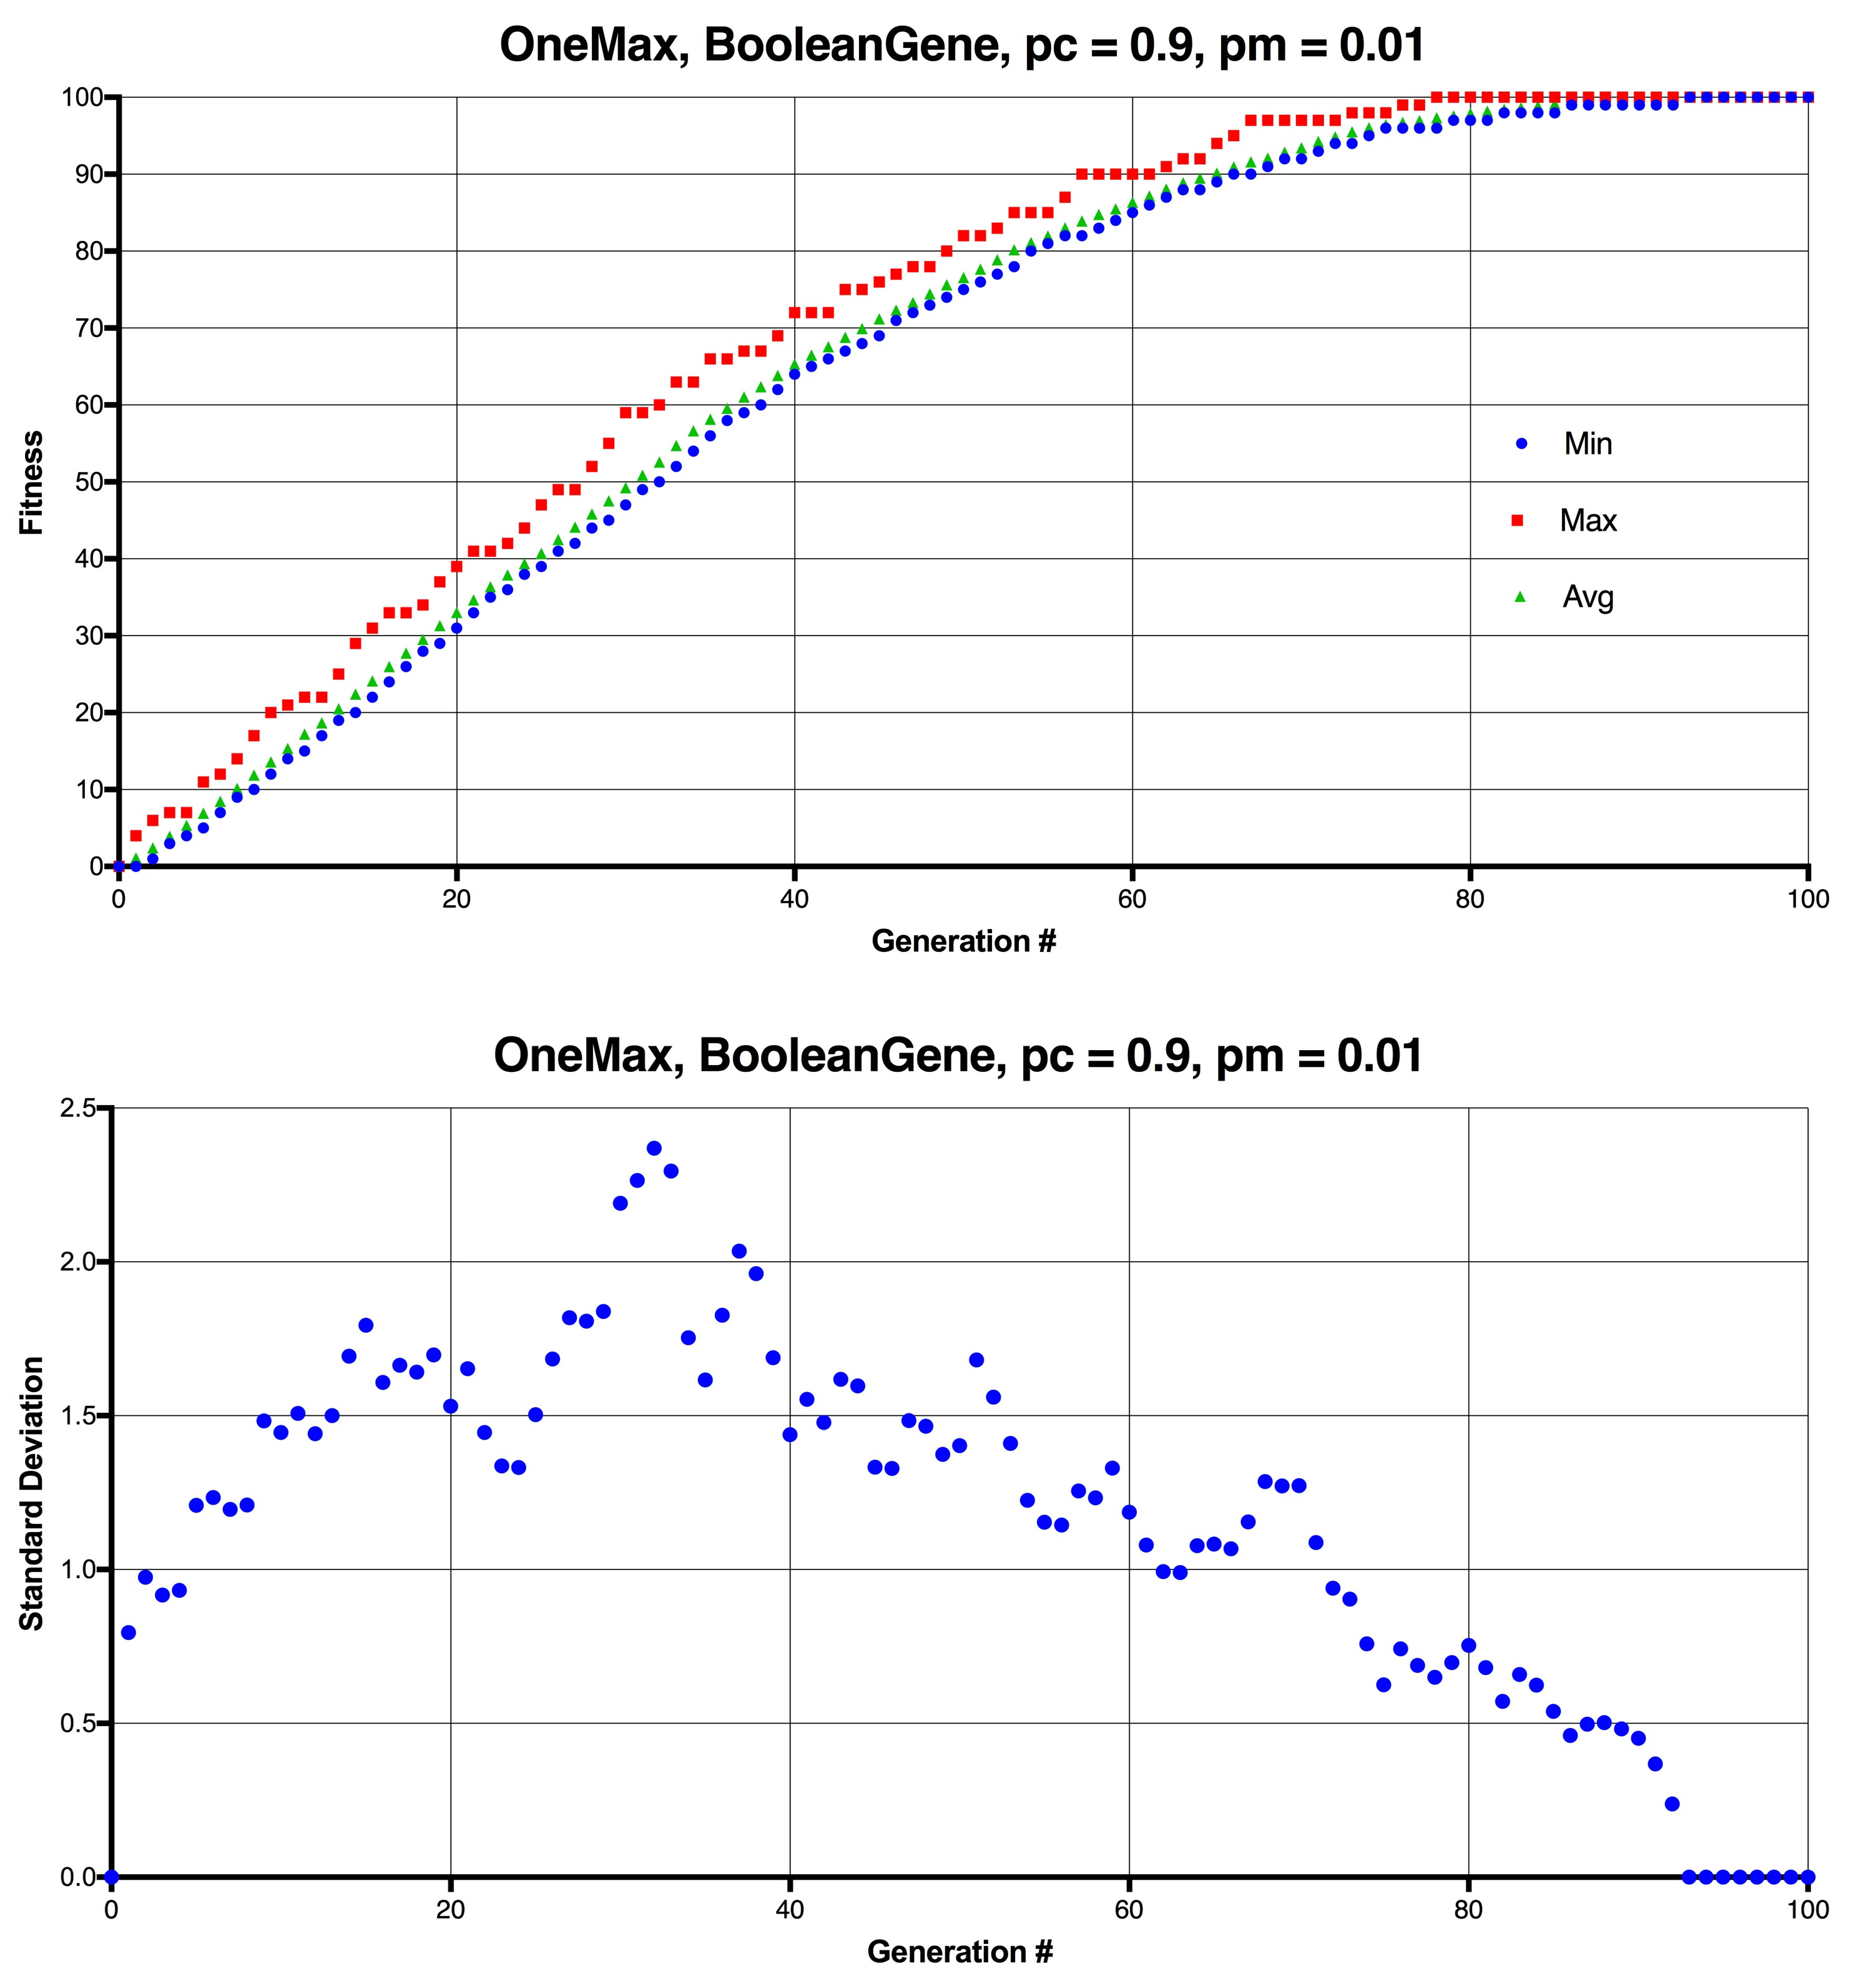
\includegraphics[width=1.0\textwidth]{onemax_boolean.jpg}
    \caption{Evolução do fitness para o problema do OneMax Booleano com mínimo, máximo e valor médio, com $p_c=0.9$ e $p_m=0.01$.}
    \label{fig:onemax_boolean}
\end{figure}

\begin{figure}[ht!]
    \centering 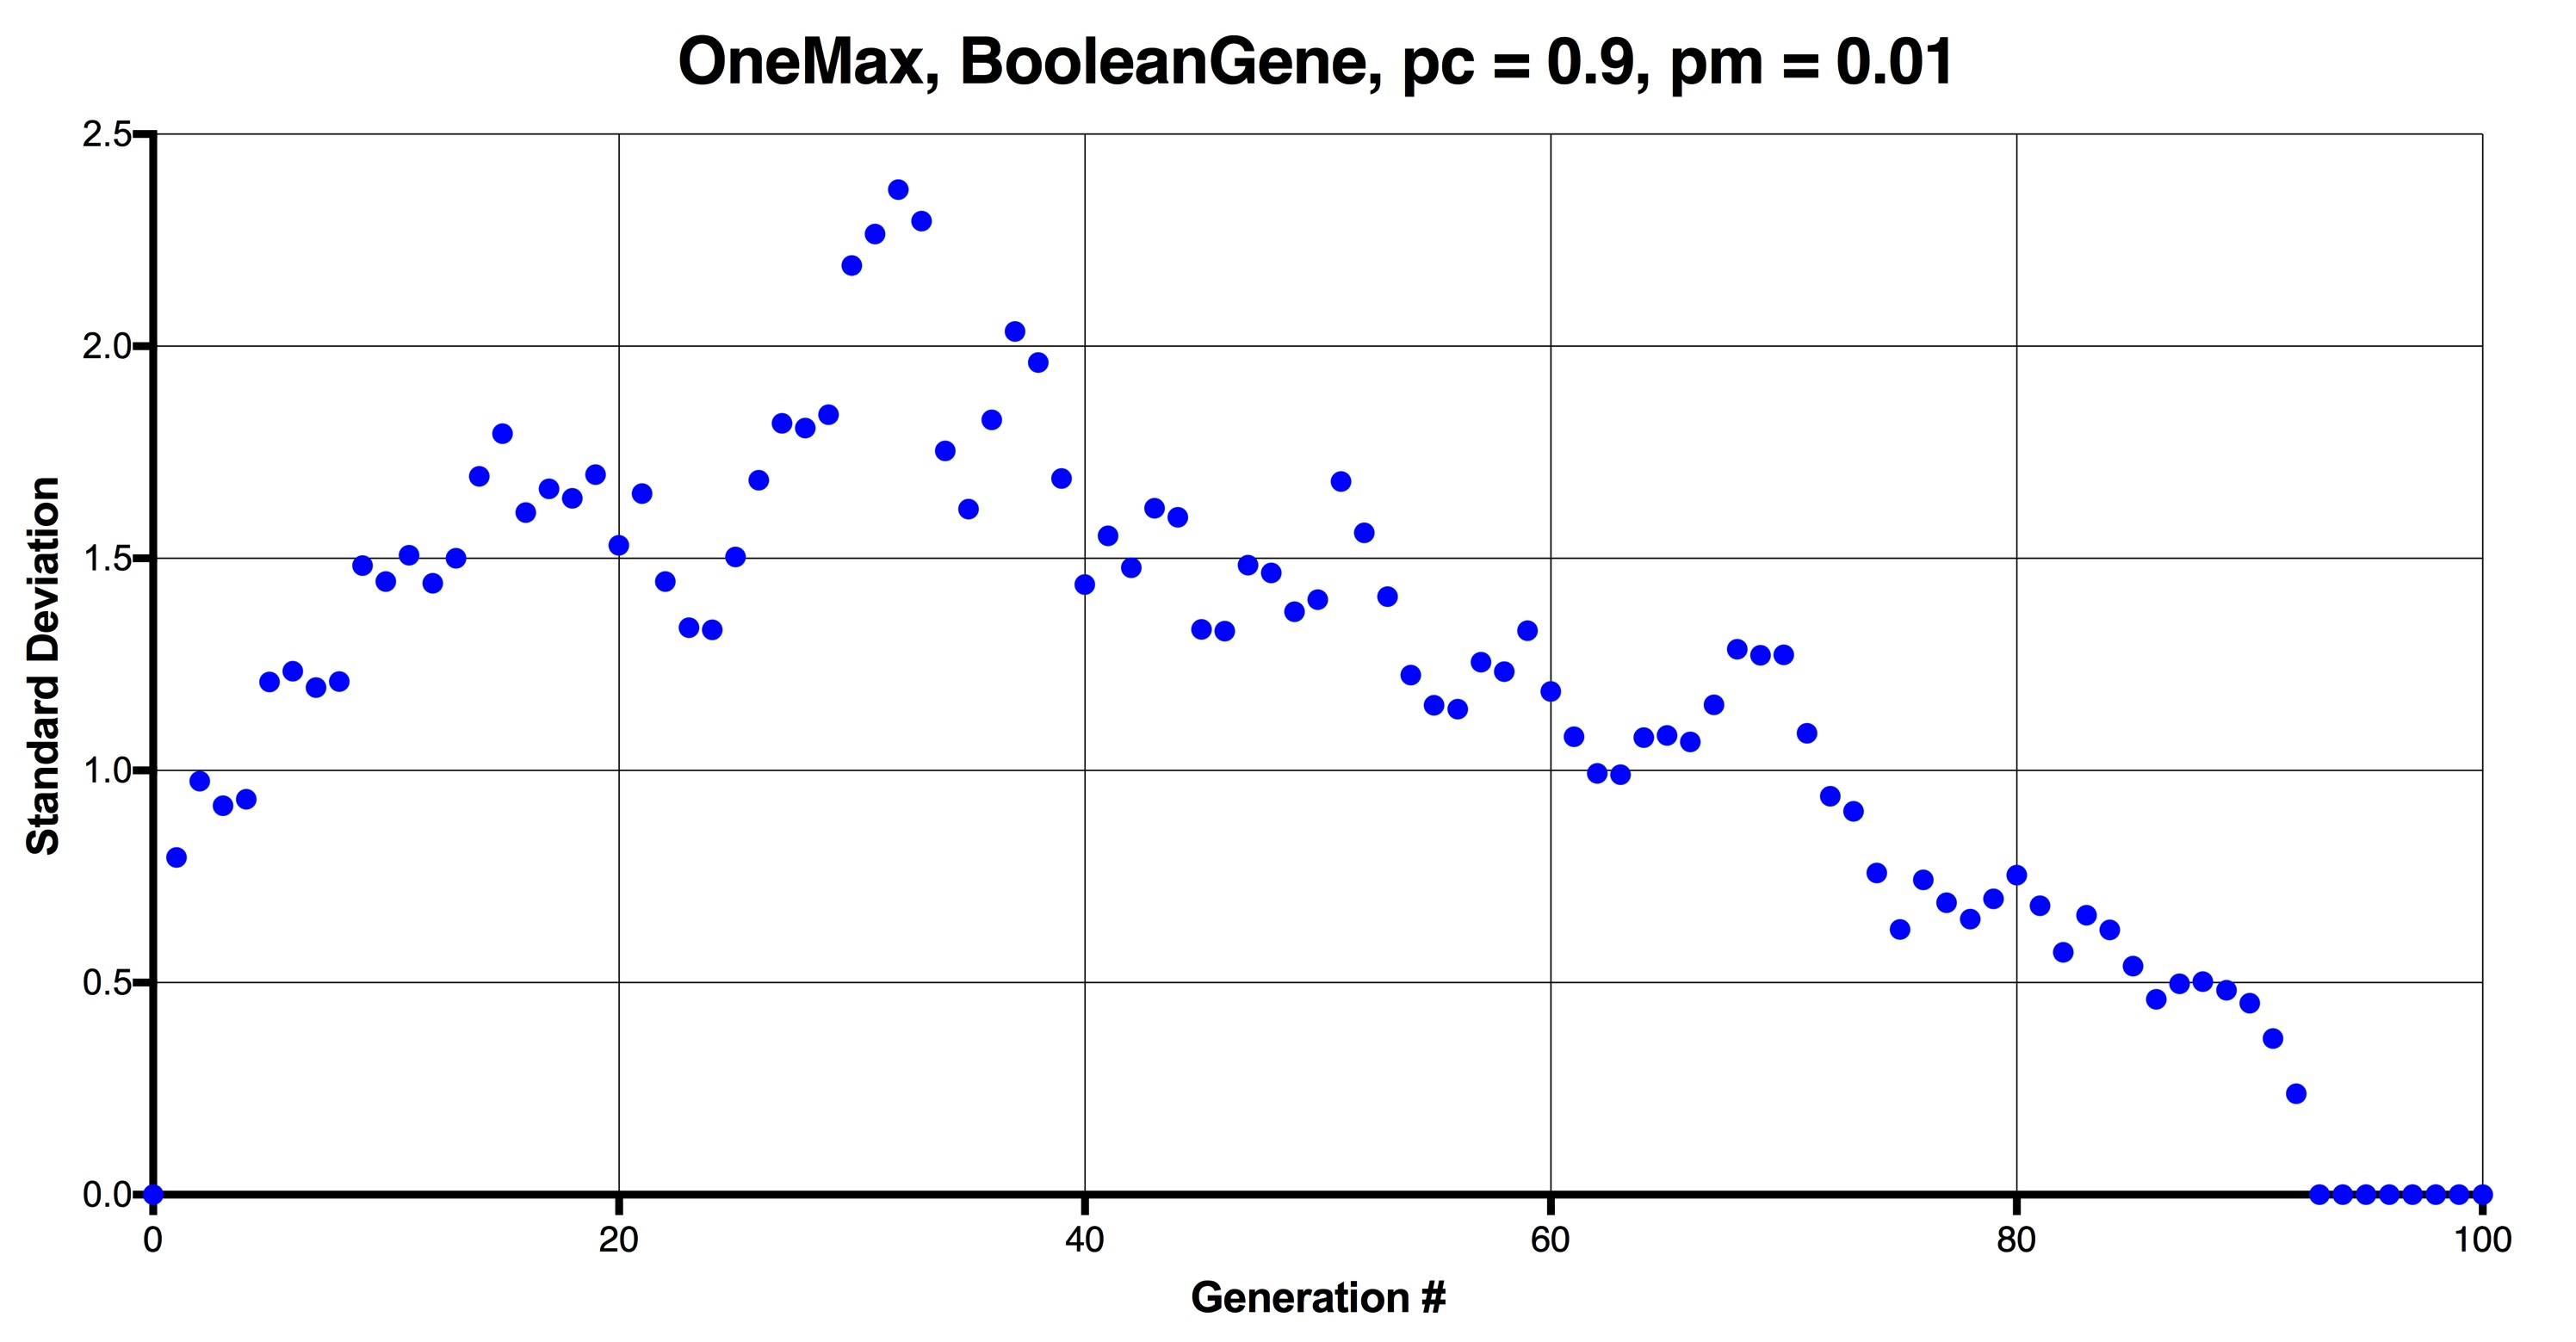
\includegraphics[width=1.0\textwidth]{onemax_boolean_std.jpg}
    \caption{Desvio padrão ao longo das gerações para o problema do OneMax Booleano, com $p_c=0.9$ e $p_m=0.01$.}
    \label{fig:onemax_boolean}
\end{figure}

\section{OneMax Real}

Texto.

\begin{figure}[ht!]
    \centering 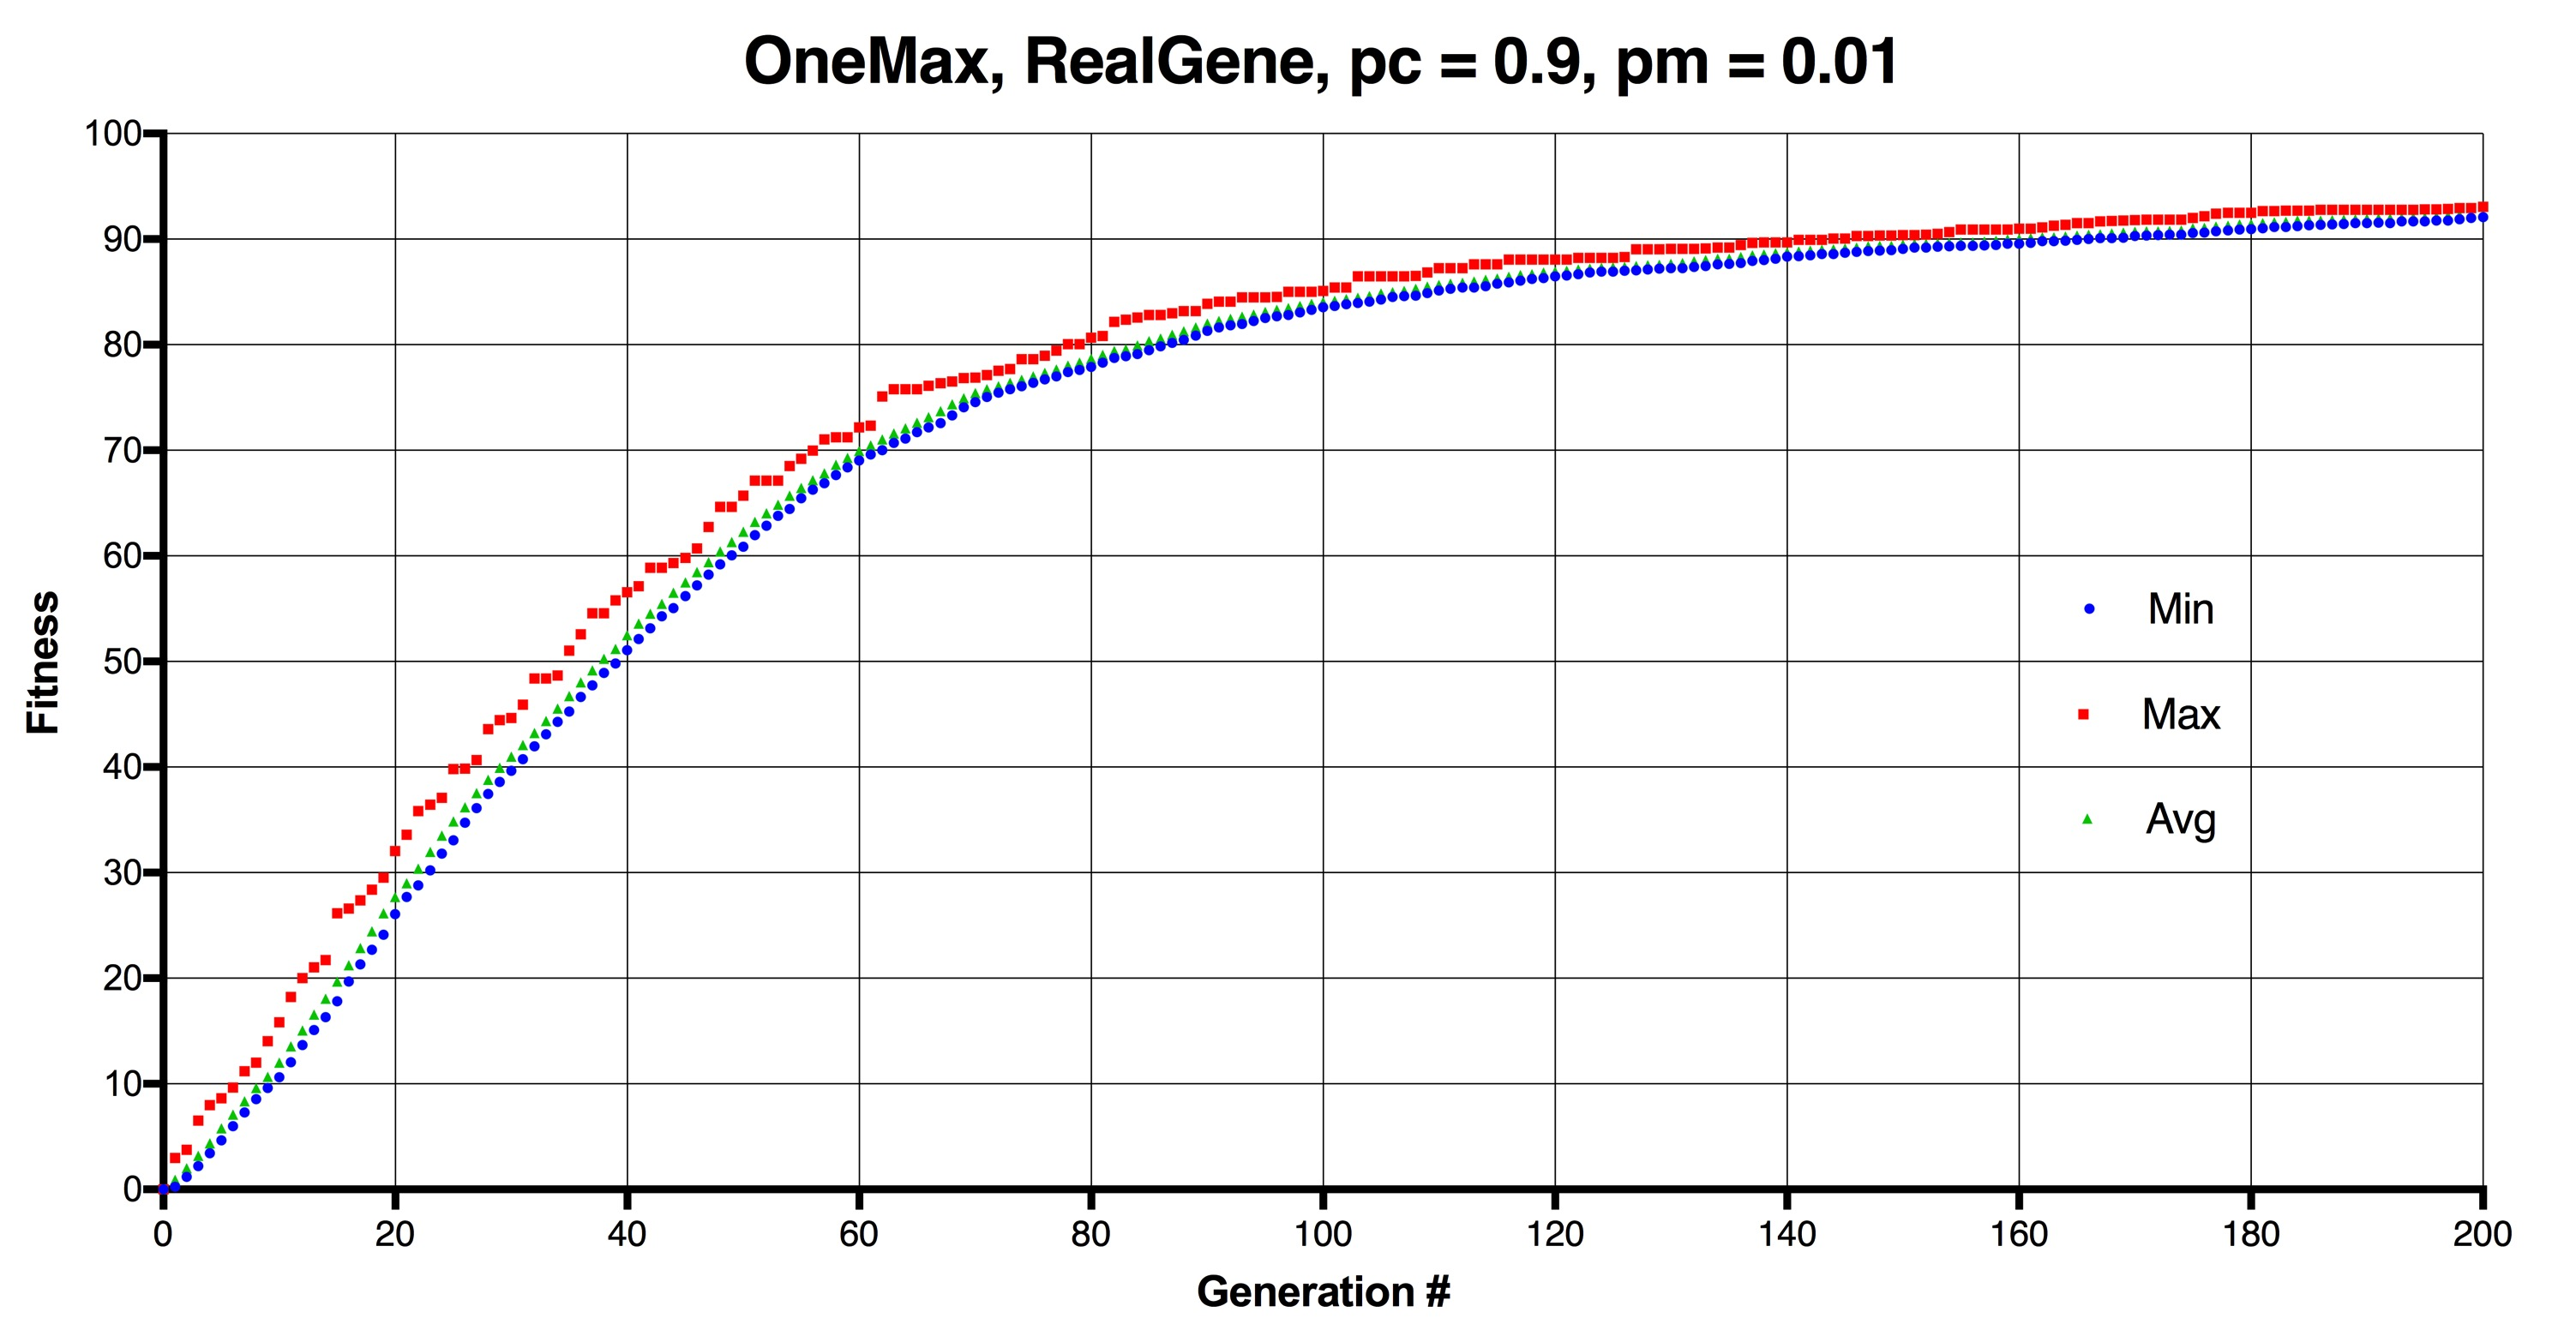
\includegraphics[width=1.0\textwidth]{onemax_real.jpg}
    \caption{Evolução do fitness para o problema do OneMax Real com mínimo, máximo e valor médio, com $p_c=0.9$ e $p_m=0.01$.}
    \label{fig:onemax_boolean}
\end{figure}

\begin{figure}[ht!]
    \centering 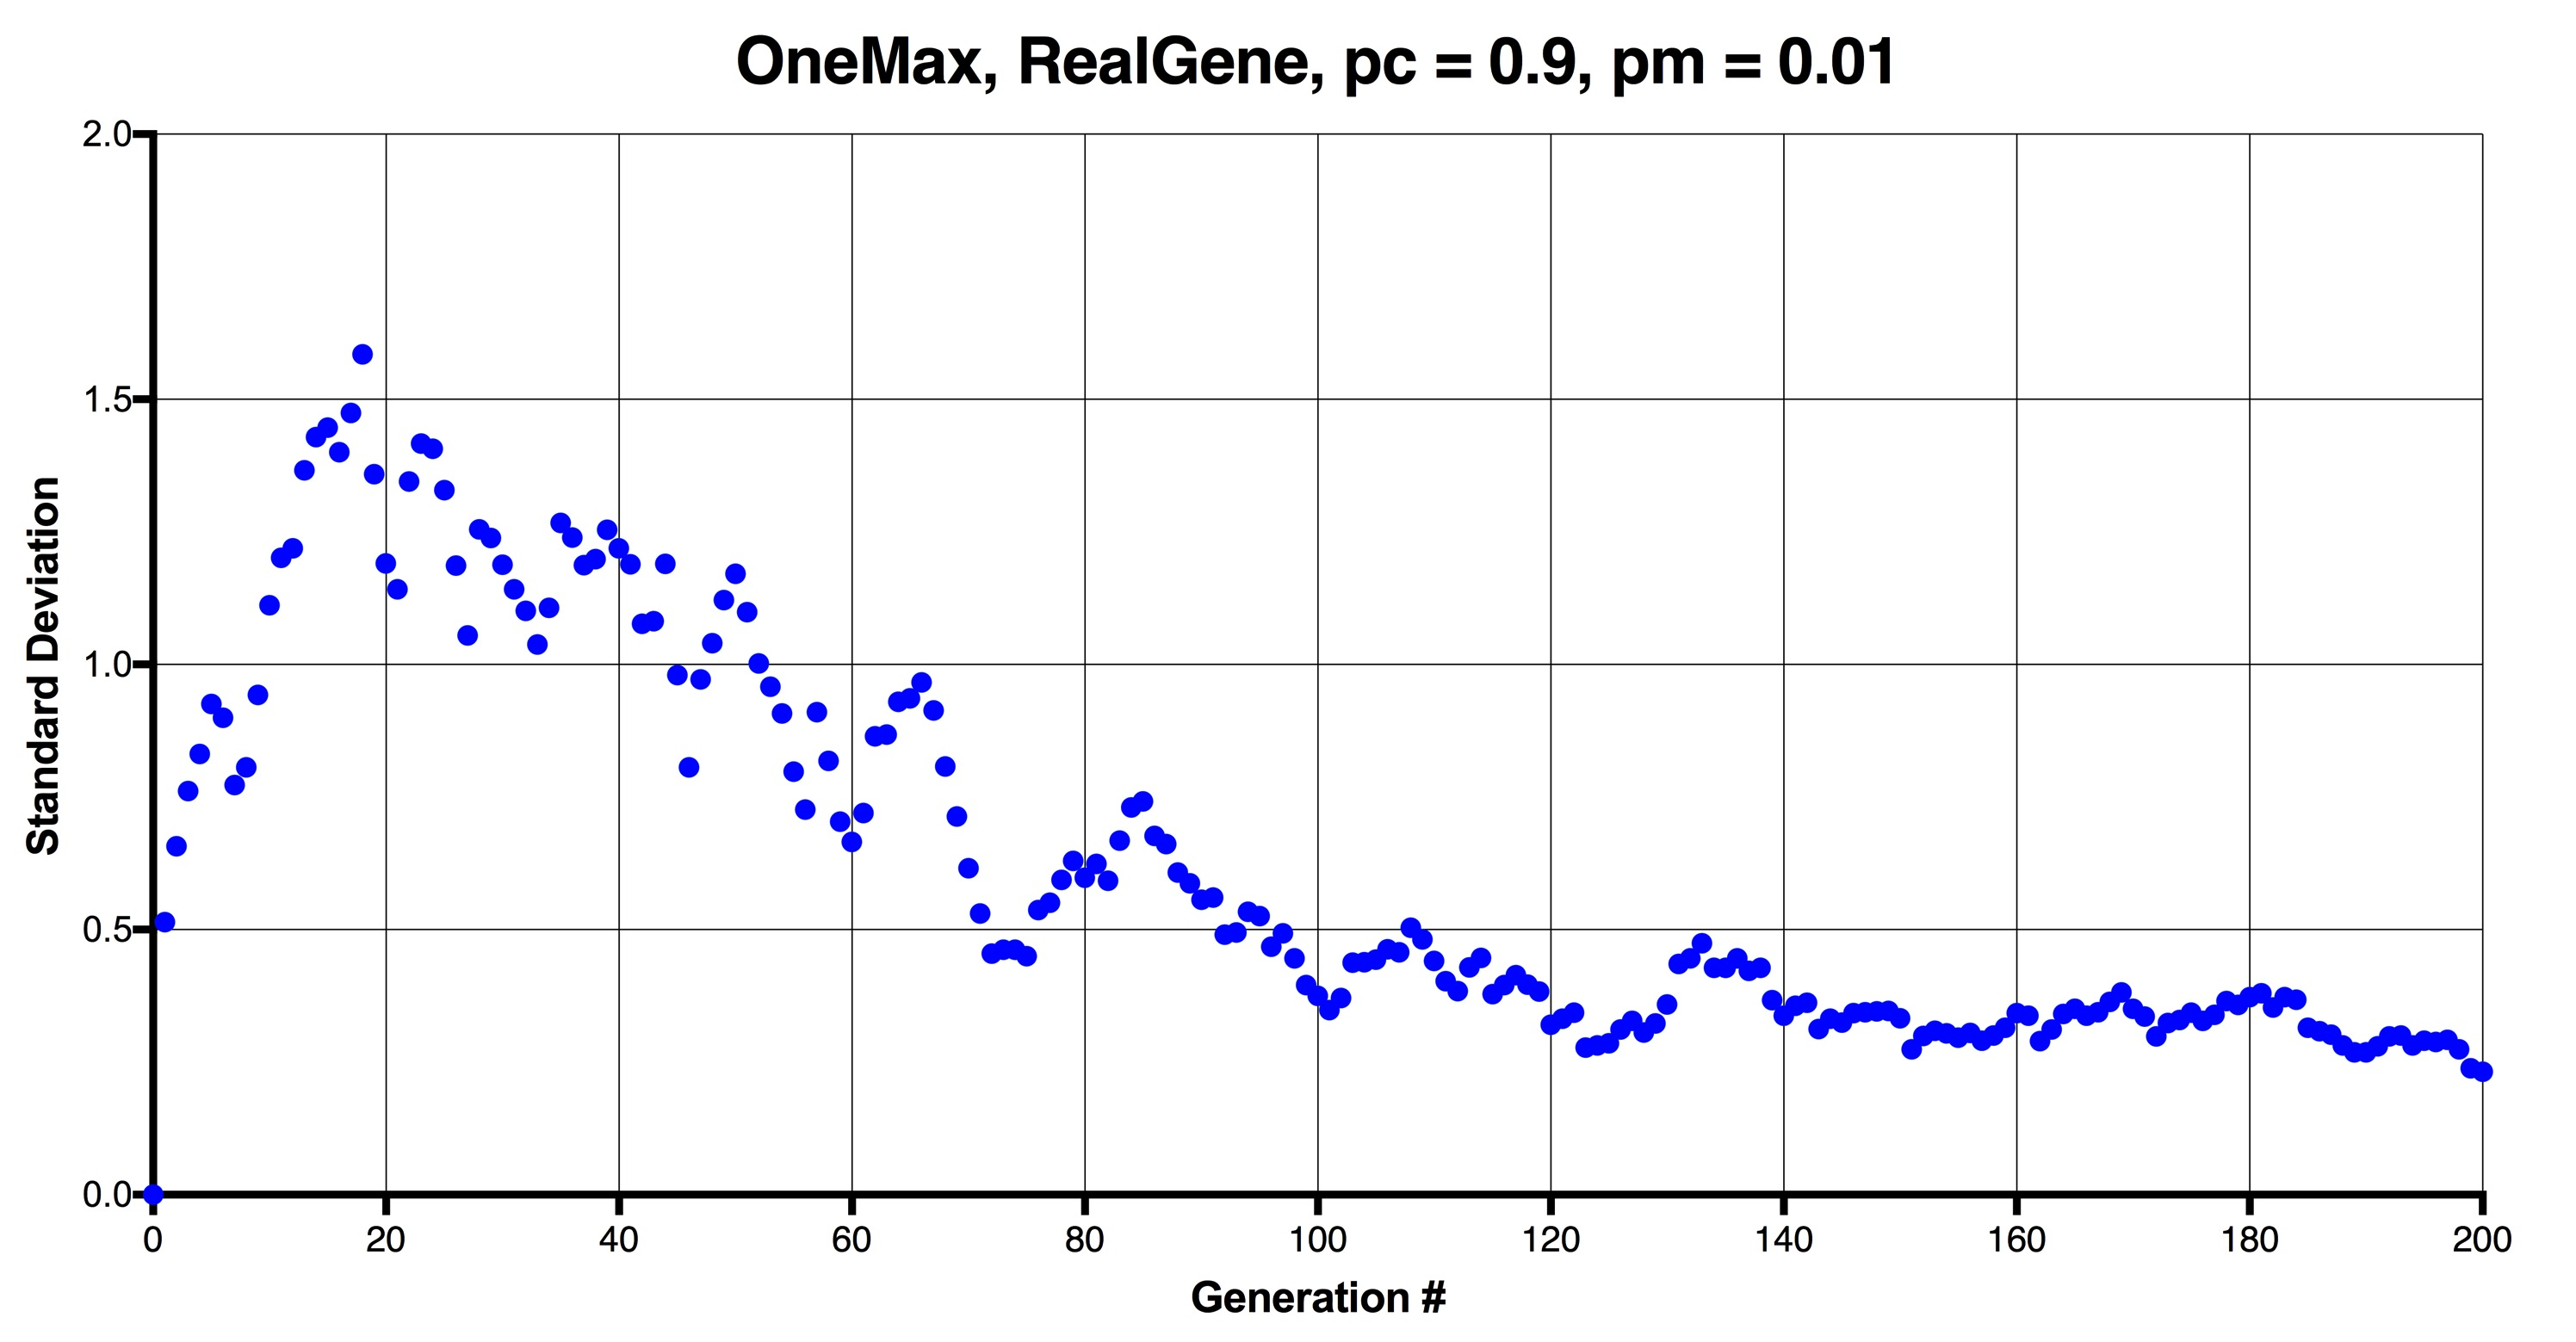
\includegraphics[width=1.0\textwidth]{onemax_real_std.jpg}
    \caption{Desvio padrão ao longo das gerações para o problema do OneMax Real, com $p_c=0.9$ e $p_m=0.01$.}
    \label{fig:onemax_boolean}
\end{figure}

\section{Caixeiro Viajante Adaptado}

Texto.

\begin{lstlisting}[float, floatplacement=H, caption={Mapa de cidades para o problema do Caixeiro Viajante Adaptado.}, label=lst:cidades]
[0, 633, 257, 91, 412, 150, 80, 134, 259, 505, 353, 324, 70, 211, 268, 246, 121],
[633, 0, 390, 661, 227, 488, 572, 530, 555, 289, 282, 638, 567, 466, 420, 745, 518],
[257, 390, 0, 228, 169, 112, 196, 154, 372, 262, 110, 437, 191, 74, 53, 472, 142],
[91, 661, 228, 0, 383, 120, 77, 105, 175, 476, 324, 240, 27, 182, 239, 237, 84],
[412, 227, 169, 383, 0, 267, 351, 309, 338, 196, 61, 421, 346, 243, 199, 528, 297],
[150, 488, 112, 120, 267, 0, 63, 34, 264, 360, 208, 329, 83, 105, 123, 364, 35],
[80, 572, 196, 77, 351, 63, 0, 29, 232, 444, 292, 297, 47, 150, 207, 332, 29],
[134, 530, 154, 105, 309, 34, 29, 0, 249, 402, 250, 314, 68, 108, 165, 349, 36],
[259, 555, 372, 175, 338, 264, 232, 249, 0, 495, 352, 95, 189, 326, 383, 202, 236],
[505, 289, 262, 476, 196, 360, 444, 402, 495, 0, 154, 578, 439, 336, 240, 685, 390],
[353, 282, 110, 324, 61, 208, 292, 250, 352, 154, 0, 435, 287, 184, 140, 542, 238],
[324, 638, 437, 240, 421, 329, 297, 314, 95, 578, 435, 0, 254, 391, 448, 157, 301],
[70, 567, 191, 27, 346, 83, 47, 68, 189, 439, 287, 254, 0, 145, 202, 289, 55],
[211, 466, 74, 182, 243, 105, 150, 108, 326, 336, 184, 391, 145, 0, 57, 426, 96],
[268, 420, 53, 239, 199, 123, 207, 165, 383, 240, 140, 448, 202, 57, 0, 483, 153],
[246, 745, 472, 237, 528, 364, 332, 349, 202, 685, 542, 157, 289, 426, 483, 0, 336],
[121, 518, 142, 84, 297, 35, 29, 36, 236, 390, 238, 301, 55, 96, 153, 336, 0]
\end{lstlisting}